\let\negthickspace\undefined
\documentclass[journal,12pt,twocolumn]{IEEEtran}
\usepackage{cite}
\usepackage{amsmath,amssymb,amsfonts,amsthm}
\usepackage{algorithmic}
\usepackage{graphicx}
\usepackage{textcomp}
\usepackage{xcolor}
\usepackage{txfonts}
\usepackage{listings}
\usepackage{enumitem}
\usepackage{mathtools}
\usepackage{gensymb}
\usepackage{comment}
\usepackage[breaklinks=true]{hyperref}
\usepackage{tkz-euclide} 
\usepackage{listings}
\usepackage{gvv}                                        
\def\inputGnumericTable{}                                 
\usepackage[latin1]{inputenc}                                
\usepackage{color}                                            
\usepackage{array}                                            
\usepackage{longtable}                                       
\usepackage{calc}                                             
\usepackage{multirow}                                         
\usepackage{hhline}                                           
\usepackage{ifthen}                                           
\usepackage{lscape}
\setlength{\arrayrulewidth}{0.5mm}
\setlength{\tabcolsep}{18pt}
\renewcommand{\arraystretch}{1.5}
\newtheorem{theorem}{Theorem}[section]
\newtheorem{problem}{Problem}
\newtheorem{proposition}{Proposition}[section]
\newtheorem{lemma}{Lemma}[section]
\newtheorem{corollary}[theorem]{Corollary}
\newtheorem{example}{Example}[section]
\newtheorem{definition}[problem]{Definition}
\newcommand{\BEQA}{\begin{eqnarray}}
\newcommand{\EEQA}{\end{eqnarray}}
\newcommand{\define}{\stackrel{\triangle}{=}}
\theoremstyle{remark}
\newtheorem{rem}{Remark}
\begin{document}
\title{Progressions (7) 11.9.5}
\author{EE23BTECH11051-Rajnil Malviya}
\date{January 2024}
\maketitle
\subsection*{\textit{Question :-}}
If a function Satisfying f\brak {x+y} = f\brak{x} f\brak{y} for all $x,y \in {N}$ such that f\brak {1} =3 and $\sum_{x=1}^{n} f\brak{x} = 120$ , find the value of n .\\
\textit{Solution:- }
\begin{align}
    y&=1\\
    \frac{f\brak{x+1}}{f\brak x}&=3
\end{align}
\begin{table}[h!]
        \begin{tabular}{ | m{1.0cm} | m{3cm} |m{1cm} |} 
  \hline
 Symbol &Description& Value \\ 
 \hline
$x(0)$&first term& 3  \\
\hline
$r$&common ratio & 3  \\
\hline
$y\brak n$& sum of all terms&120 \\
\hline
$x(n)$&n term&  depends on n\\
\hline
\end{tabular}\\
\caption{}
\label{Table:1}    
    \end{table}
\begin{align}
x \brak n = x \brak 0r^{n}u\brak n
\label{eq:11.9.5.7}
\end{align}
From \eqref{eq:11.9.5.7}
\begin{align}
X(z) &=\frac{3}{1-3z^{-1}} \quad \abs{z} > \abs{3}
\end{align}


\begin{align}
Y(z)&=\frac{X\brak0}{r-1}\brak{\frac{r}{1-r z^{-1}}-\frac{1}{1- z^{-1}}}  \quad \abs{z} > \abs{r}
\end{align}
inverse of above can be expressed as 
\begin{align}
y(n) &= x(0)\brak{\frac{r^{n+1}-1}{r-1}}u(n)\\
120 &= 3\brak{ \frac{3^{n+1}- 1}{3-1}}  \\
\implies n &= 3
\end{align}
\begin{figure}
   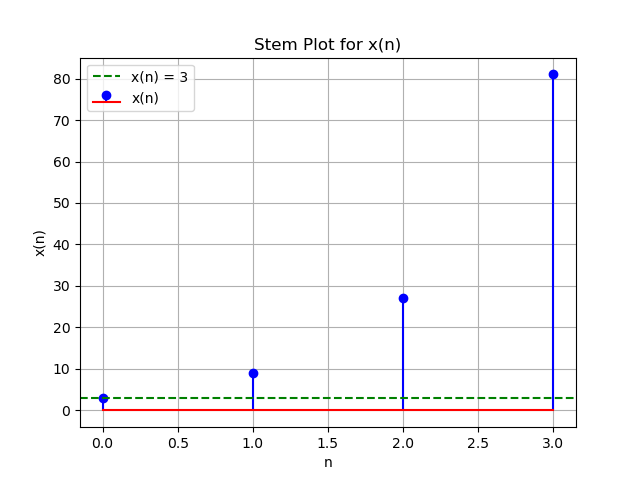
\includegraphics[width=1\linewidth]{figs/i1.png}
\end{figure}
\begin{figure}
   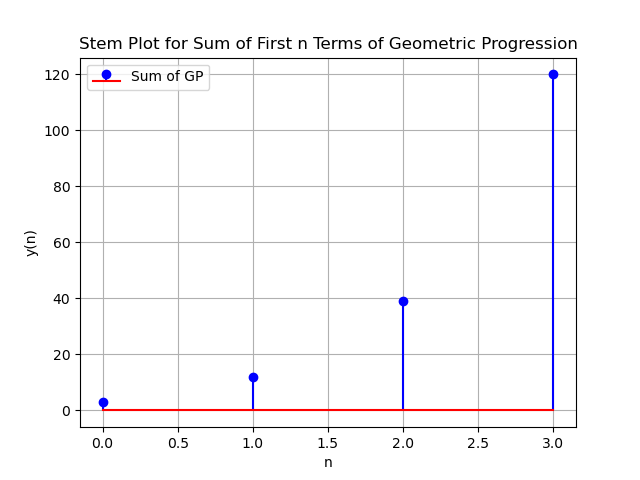
\includegraphics[width=1\linewidth]{figs/i2.png}
\end{figure}
\end{document}
